%%%%%%%%%%%%%%%%%%%%%%%%%%%%%%%%%%%%%%%%%
% Arsclassica Article
% LaTeX Template
% Version 1.1 (10/6/14)
%
% This template has been downloaded from:
% http://www.LaTeXTemplates.com
%
% Original author:
% Lorenzo Pantieri (http://www.lorenzopantieri.net) with extensive modifications by:
% Vel (vel@latextemplates.com)
%
% License:
% CC BY-NC-SA 3.0 (http://creativecommons.org/licenses/by-nc-sa/3.0/)
%
%%%%%%%%%%%%%%%%%%%%%%%%%%%%%%%%%%%%%%%%%

%----------------------------------------------------------------------------------------
%	PACKAGES AND OTHER DOCUMENT CONFIGURATIONS
%----------------------------------------------------------------------------------------

\documentclass[
10pt, % Main document font size
a4paper, % Paper type, use 'letterpaper' for US Letter paper
oneside, % One page layout (no page indentation)
%twoside, % Two page layout (page indentation for binding and different headers)
headinclude,footinclude, % Extra spacing for the header and footer
BCOR5mm, % Binding correction
]{scrartcl}

%%%%%%%%%%%%%%%%%%%%%%%%%%%%%%%%%%%%%%%%%
% Arsclassica Article
% Structure Specification File
%
% This file has been downloaded from:
% http://www.LaTeXTemplates.com
%
% Original author:
% Lorenzo Pantieri (http://www.lorenzopantieri.net) with extensive modifications by:
% Vel (vel@latextemplates.com)
%
% License:
% CC BY-NC-SA 3.0 (http://creativecommons.org/licenses/by-nc-sa/3.0/)
%
%%%%%%%%%%%%%%%%%%%%%%%%%%%%%%%%%%%%%%%%%

%----------------------------------------------------------------------------------------
%	REQUIRED PACKAGES
%----------------------------------------------------------------------------------------

\usepackage[
nochapters, % Turn off chapters since this is an article        
beramono, % Use the Bera Mono font for monospaced text (\texttt)
eulermath,% Use the Euler font for mathematics
pdfspacing, % Makes use of pdftex’ letter spacing capabilities via the microtype package
dottedtoc % Dotted lines leading to the page numbers in the table of contents
]{classicthesis} % The layout is based on the Classic Thesis style

\usepackage{arsclassica} % Modifies the Classic Thesis package

\usepackage[T1]{fontenc} % Use 8-bit encoding that has 256 glyphs

\usepackage[utf8]{inputenc} % Required for including letters with accents

\usepackage{graphicx} % Required for including images
\graphicspath{{Figures/}} % Set the default folder for images

\usepackage{enumitem} % Required for manipulating the whitespace between and within lists

\usepackage{lipsum} % Used for inserting dummy 'Lorem ipsum' text into the template

\usepackage{subfig} % Required for creating figures with multiple parts (subfigures)

\usepackage{amsmath,amssymb,amsthm} % For including math equations, theorems, symbols, etc

\usepackage{varioref} % More descriptive referencing
\usepackage{color}
\usepackage{listings}
\usepackage{setspace}

\usepackage{lscape}


%----------------------------------------------------------------------------------------
%	THEOREM STYLES
%---------------------------------------------------------------------------------------

\theoremstyle{definition} % Define theorem styles here based on the definition style (used for definitions and examples)
\newtheorem{definition}{Definition}

\theoremstyle{plain} % Define theorem styles here based on the plain style (used for theorems, lemmas, propositions)
\newtheorem{theorem}{Theorem}

\theoremstyle{remark} % Define theorem styles here based on the remark style (used for remarks and notes)

%----------------------------------------------------------------------------------------
%	HYPERLINKS
%---------------------------------------------------------------------------------------

\hypersetup{
%draft, % Uncomment to remove all links (useful for printing in black and white)
colorlinks=true, breaklinks=true, bookmarks=true,bookmarksnumbered,
urlcolor=webbrown, linkcolor=RoyalBlue, citecolor=webgreen, % Link colors
pdftitle={}, % PDF title
pdfauthor={\textcopyright}, % PDF Author
pdfsubject={}, % PDF Subject
pdfkeywords={}, % PDF Keywords
pdfcreator={pdfLaTeX}, % PDF Creator
pdfproducer={LaTeX with hyperref and ClassicThesis} % PDF producer
}

\definecolor{Code}{rgb}{0,0,0}
\definecolor{Decorators}{rgb}{0.5,0.5,0.5}
\definecolor{Numbers}{rgb}{0.5,0,0}
\definecolor{MatchingBrackets}{rgb}{0.25,0.5,0.5}
\definecolor{Keywords}{rgb}{0,0,1}
\definecolor{self}{rgb}{0,0,0}
\definecolor{Strings}{rgb}{0,0.63,0}
\definecolor{Comments}{rgb}{0,0.63,1}
\definecolor{Backquotes}{rgb}{0,0,0}
\definecolor{Classname}{rgb}{0,0,0}
\definecolor{FunctionName}{rgb}{0,0,0}
\definecolor{Operators}{rgb}{0,0,0}
\definecolor{Background}{rgb}{0.98,0.98,0.98}

\lstnewenvironment{python}[1][]{
\lstset{
numbers=left,
numberstyle=\footnotesize,
numbersep=1em,
xleftmargin=1em,
framextopmargin=2em,
framexbottommargin=2em,
showspaces=false,
showtabs=false,
showstringspaces=false,
frame=l,
tabsize=4,
% Basic
basicstyle=\ttfamily\small\setstretch{1},
backgroundcolor=\color{Background},
language=Python,
% Comments
commentstyle=\color{Comments}\slshape,
% Strings
stringstyle=\color{Strings},
morecomment=[s][\color{Strings}]{"""}{"""},
morecomment=[s][\color{Strings}]{'''}{'''},
% keywords
morekeywords={import,from,class,def,for,while,if,is,in,elif,else,not,and,or,print,break,continue,return,True,False,None,access,as,,del,except,exec,finally,global,import,lambda,pass,print,raise,try,assert},
keywordstyle={\color{Keywords}\bfseries},
% additional keywords
morekeywords={[2]@invariant},
keywordstyle={[2]\color{Decorators}\slshape},
emph={self},
emphstyle={\color{self}\slshape},
%
}}{}

 % Include the structure.tex file which specified the document structure and layout

\hyphenation{Fortran hy-phen-ation} % Specify custom hyphenation points in words with dashes where you would like hyphenation to occur, or alternatively, don't put any dashes in a word to stop hyphenation altogether



%----------------------------------------------------------------------------------------
%	TITLE AND AUTHOR(S)
%----------------------------------------------------------------------------------------

\title{\normalfont\spacedallcaps{Detecting local events in the Twitter stream}} % The article title

\author{\spacedlowsmallcaps{Chris Pool}} % The article author(s) - author affiliations need to be specified in the AUTHOR AFFILIATIONS block

\date{} % An optional date to appear under the author(s)

%----------------------------------------------------------------------------------------

\begin{document}

%----------------------------------------------------------------------------------------
%	HEADERS
%----------------------------------------------------------------------------------------

\renewcommand{\sectionmark}[1]{\markright{\spacedlowsmallcaps{#1}}} % The header for all pages (oneside) or for even pages (twoside)
%\renewcommand{\subsectionmark}[1]{\markright{\thesubsection~#1}} % Uncomment when using the twoside option - this modifies the header on odd pages
\lehead{\mbox{\llap{\small\thepage\kern1em\color{halfgray} \vline}\color{halfgray}\hspace{0.5em}\rightmark\hfil}} % The header style

\pagestyle{scrheadings} % Enable the headers specified in this block


%----------------------------------------------------------------------------------------
%	Omslag
%----------------------------------------------------------------------------------------


\begin{titlepage}

\begin{figure}[h!] %  figure placement: here, top, bottom, or page

 
\includegraphics[width=4in]{Figures/ruglogo.eps} 
\end{figure}
\begin{center}

\vspace{30 mm}
\begingroup \linespread{1,75} \selectfont 
\textsc{\LARGE Detecting local events in the Twitter stream}\\[1,5cm]
\endgroup


by\\[0,5cm]
Chris Pool\\[2,5cm]


\end{center}
\vfill
\textbf{Bachelor thesis}\\
Information sciences\\
Chris Pool\\
S2816539\\
June 14, 2015



\end{titlepage}


%----------------------------------------------------------------------------------------
%	Title page
%----------------------------------------------------------------------------------------

\maketitle % Print the title/author/date block
\begin{figure}[htbp] %  figure placement: here, top, bottom, or page
   \centering
   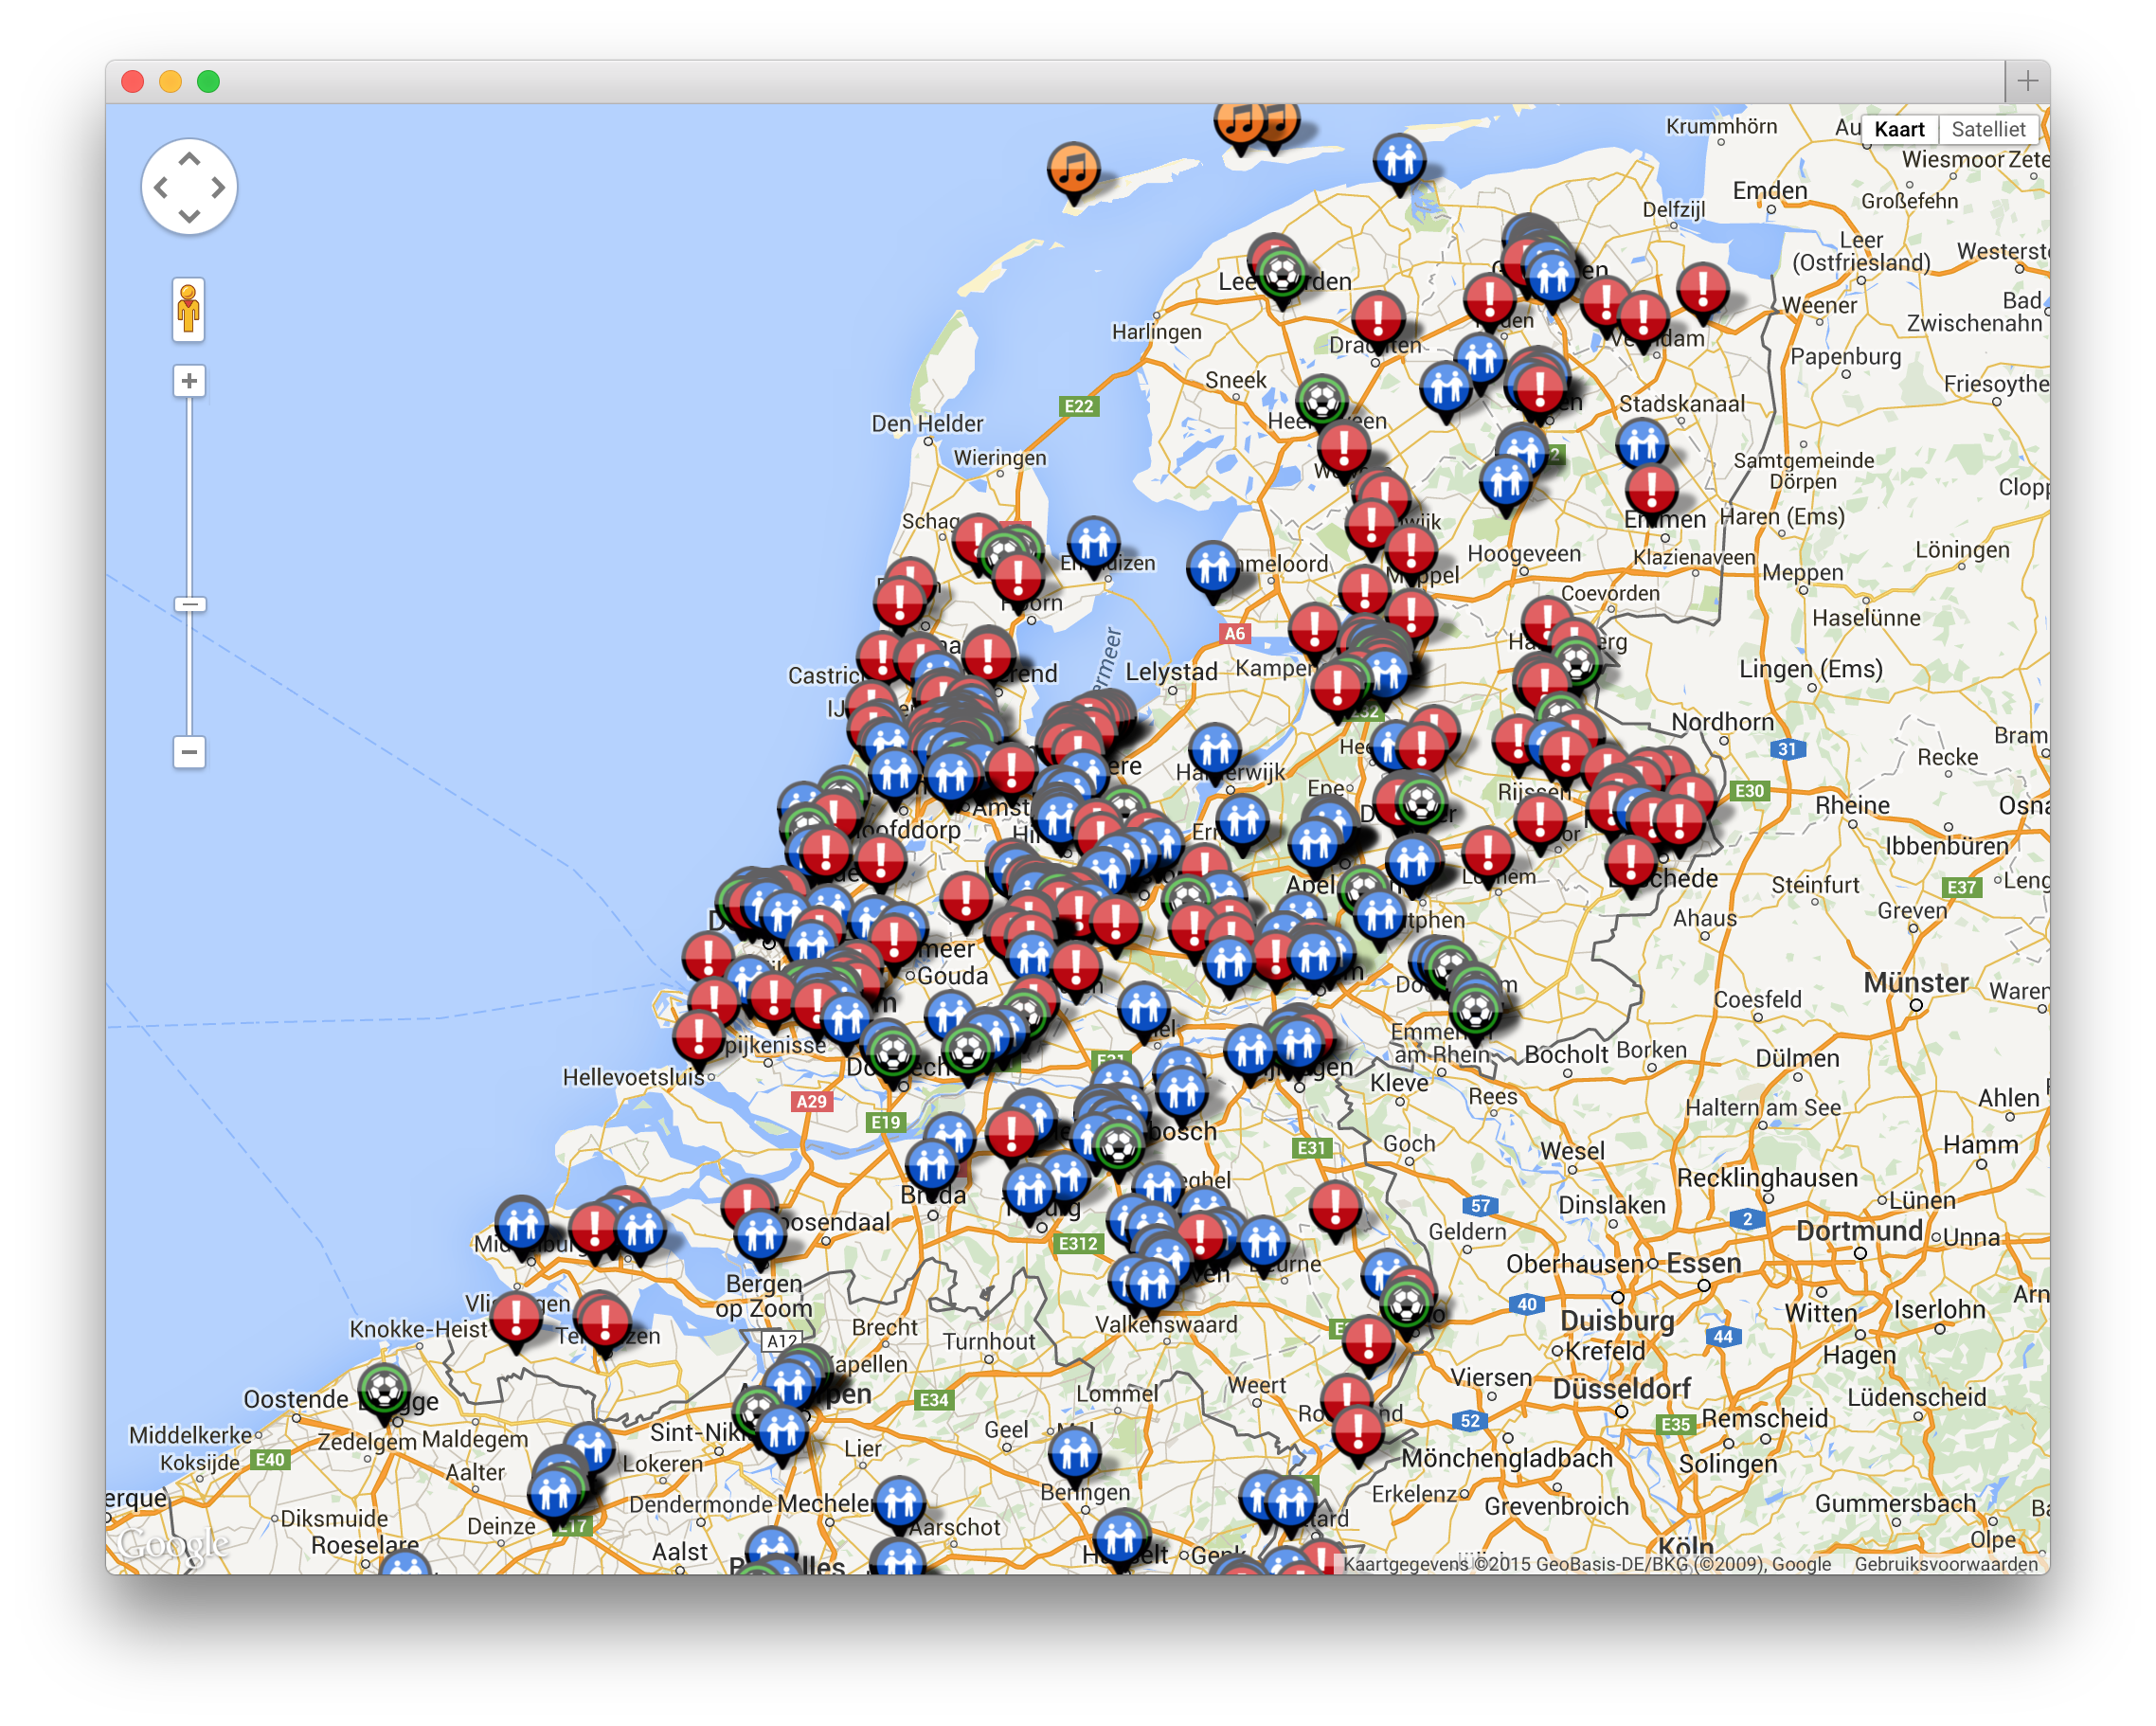
\includegraphics[width=4.5in]{voorkant.png} 
   \label{fig:gui}
\end{figure}


%----------------------------------------------------------------------------------------
%	Preface
%----------------------------------------------------------------------------------------
\newpage
\section*{Preface} % This section will not appear in the table of contents due to the star (\section*)




%----------------------------------------------------------------------------------------
%	TABLE OF CONTENTS & LISTS OF FIGURES AND TABLES
%----------------------------------------------------------------------------------------
\newpage
\setcounter{tocdepth}{2} % Set the depth of the table of contents to show sections and subsections only
\tableofcontents % Print the table of contents

\listoffigures % Print the list of figures

\listoftables % Print the list of tables

%----------------------------------------------------------------------------------------
%	ABSTRACT
%----------------------------------------------------------------------------------------
\newpage
\section*{Abstract} % This section will not appear in the table of contents due to the star (\section*)

\lipsum[1] % Dummy text


%----------------------------------------------------------------------------------------

\newpage % Start the article content on the second page, remove this if you have a longer abstract that goes onto the second page

%----------------------------------------------------------------------------------------
%	INTRODUCTION
%----------------------------------------------------------------------------------------

\section{Introduction}

%waarom
With the growing number of people using social media services like Twitter and the enormous amount of data available makes it interesting to use as a source of information about events that are taking place at a certain time and location. This real-time information in combination with user sentiment can be very informative, for example to provide news items with more information about the opinion of people present.

%wat
This thesis describes a method of finding local events based on tweets with geo-information and categorize them into 5 categories (No-event, Sport, Entertainment, Meeting and Incident) and to find relevant information within those tweets about the location and people involved. Local events are events that take place in a certain radius (\begin{math}Z\end{math}) within a certain time interval (\begin{math}X\end{math}). For this research \begin{math}z= 0.5km , x= 5 hours\end{math}.

My research question is: Is it possible to detect local events from the Twitter stream that take place in the Netherlands based on Tweets with geo-information, to see if you can detect what type of events take place and who the important people/organizations or topics are to make an interactive map of these events.

%hoe
You can find in the first chapter the discussion of existing research. In the second chapter I describe the techniques that i use for my research and in the final chapter my experiment and results.

%----------------------------------------------------------------------------------------
%	Related literature
%----------------------------------------------------------------------------------------
\newpage
\section{Related literature}
Walter and Kaisser[1] describe in their paper Geo-spatial event detection in the Twitter stream a way to recognize geo-spatial events. They focus on small events that take place in a small area like fires and traffic jams. It differs from my research because I want to focus on locations where events of different sizes can take place but the features they use can be useful for my research. Especially how they calculate the clusterscore (cluster of tweets from a region) can be useful. Unfortunately they do not describe how they make clusters of locations.

Amineh Amini et al.: Density-Based Data Streams Clustering Survey[2] is a paper about different clustering techniques and is interesting to see which ones I can use to make clusters of the locations and the events. DBSCAN is one of the density-based clustering algorithms I maybe can use.  DBSCAN (Density-Based Spatial Clustering of Applications with Noise) is developed for clustering large spatial databases with noise, based on connected regions with high density. The density of each point is defined based on the number of points close to that particular point called the point's neighborhood.
The dense neighborhood is defined based on two user-specified parameters: the radius (of the neighborhood, and the number of the objects in the neighborhood 




%----------------------------------------------------------------------------------------
%	METHOD
%----------------------------------------------------------------------------------------
\newpage
\section{Method}
In this chapter the used methods for the experiment are described. 

\subsection{Clustering}
The first task is to cluster the tweets based on their location and the time the tweets are published. There are several approaches in location clustering that can be used as discussed in the previous chapter. Because the aim of the research was to make something that could work in real-time it was necessary to look for an approach that was quick. GeoHash is is a system invented by Gustavo Niemeyer \cite{geohash} that converts latitude and longitude coordinates into a \textit{geoHash}. The hash represents an area where in the location is present. The more digits used indicates a smaller area, and thus a higher precision. If two locations share the same prefix it indicates (not always) that the locations are nearby. 

\begin{figure}[htbp] %  figure placement: here, top, bottom, or page
   \centering
   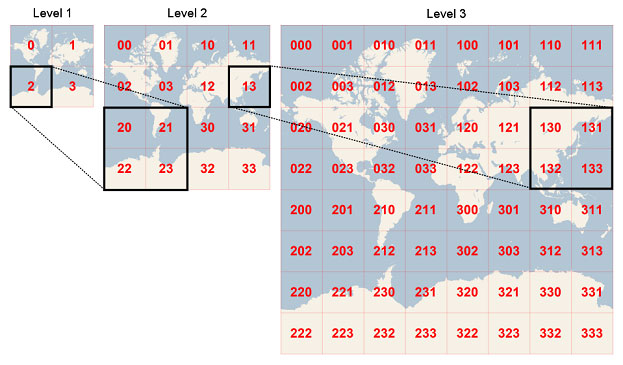
\includegraphics[width=4.5in]{geohash.jpg} 
   \caption{Geohash}
   \label{fig:geohash}
\end{figure}
Figure 1 illustrates how geoHash works. The first digit indicates which halve of the earth the area is on. The second digit divides that area in four areas and that continues resulting in the table below that show the different lengths of the \textit{geoHash} and the accuracy of that length. Because the dimensions of the area are different at each latitude the values represent the worst-case scenario at the equator.


\begin{table}[h]
\caption[Geohash Precision]{Geohash Precision \cite{elasticsearch} }
\begin{tabular}{|c|c|}
\hline
GeoHash length & Area width x height   \\ \hline
1              & 5,009.4km x 4,992.6km \\ \hline
2              & 1,252.3km x 624.1km   \\ \hline
3              & 156.5km x 156km       \\ \hline
4              & 39.1km x 19.5km       \\ \hline
5              & 4.9km x 4.9km         \\ \hline
6              & 1.2km x 609.4m        \\ \hline
7              & 152.9m x 152.4m       \\ \hline
8              & 38.2m x 19m           \\ \hline
9              & 4.8m x 4.8m           \\ \hline
10             & 1.2m x 59.5cm         \\ \hline
11             & 14.9cm x 14.9cm       \\ \hline
12             & 3.7cm x 1.9cm         \\ \hline
\end{tabular}
\end{table}

\newpage
There are several implementations of this algorithm in Python. I used the GeoHash library written in 2009 by Hiroaki Kawai\cite{geohash-module} because of the good documentation and excellent features. The function to calculate the \textit{geoHash} of a location requires the desired accuracy, latitude and longitude of that location and returns the \textit{geoHash} for that location. 

\begin{python}
lon = 52.348
lat = 6.2342
accuracy = 7

hash = geohash.encode(lon,lat,accuracy)
>>> print(hash)
u1k3y1c
\end{python}

The library also provides functions to calculate the neighboring geoHashes, this is useful because in a grid clustering approach border cases can occur.  This  functionality can be used to merge those border cases. \newline

For clustering based on time the UNIX timestamp can be used. That is a system to represent time using the number of seconds since 1 January 1970. Python has build-in functions to deal with UNIX timestamps. The tweets are sorted on timestamp making it easy to make clusters of time series.


\subsection{NLTK}
Python has a lot of functions to use while doing NLP tasks but for more advanced tasks it is not powerful enough. Therefore I have chosen to use the Natural Language Tookit (NLTK)\cite{NTLK-website}%link naar bron.
NLTK has a lot of modules that can be used for a wide range of NLP tasks. It is also really easy to use and well documented. Another advantage is that NLTK is modular, meaning you can use small portions of the toolkit that work together with other libraries. 


\subsection{Classification}
After forming the potential events (\textit{Event Candidates}) the Event Candidates have to be classified as a specific event category or not an event.  NLTK provides excellent documentation and functions for classifying. \newline  NLTK enables you to use several classifiers:

\begin{itemize}[noitemsep]
\item ConditionalExponentialClassifier
\item DecisionTreeClassifier
\item MaxentClassifier
\item NaiveBayesClassifier
\item WekaClassifier
\item SVMClassifier (using scikit-learn)
\end{itemize}

In my experiment I have chosen to use the MaxEntClassifier, NaiveBayes and a SVM classifier. Training the different classifiers is easily done with NLTK. The format of the training file is the same for the different classifiers. Also functions to calculate accuracy, precision and recall are standard NLTK functions. I tested these three classifiers because their different approaches.

\newpage
\subsection{Named Entity Reconinigzion}
For finding the important persons, organizations and locations I want to use Named Entity Reconinigzion(NER). NER is the proces of labeling data with corresponding categories like person, organization or location. For example:

\begin {quote}
Klaar voor \textbf{Ajax(organization)} - \textbf{NAC(organization)} @\textbf{Amsterdam(location)} @\textbf{ArenAPoort(location) }in \textbf{Amsterdam(location)} Zuidoost, \textbf{Noord-Holland(location)}
\end{quote}

Current NER tools were designed to process large texts and perform poorly with tweets due to the noisy and short style of tweets. One of the most used NER tools is Stanford NER. This Java implementation is also known as CRFClassifier. The software comes with 3 trained classifiers that perform particularly well for the three classes persons, organizations and locations. Some experiments are done with using labeled tweets as train data but mostly in English.

Because there is no classifier trained with Dutch tweets I want to train my own classifier that I describe in detail in the next chapter.


%----------------------------------------------------------------------------------------
%	Experiment and Evaluation
%----------------------------------------------------------------------------------------
\newpage
\section{Experiment and Evaluation}
For my experiment I worked together with David de Kleer in collecting the data and building the Python modules. The goal was to build a system that can detect events that take place at a specific location, for example concerts, football matches, fires and traffic jams and recognize the named entities in the tweets.  Events that take place on a larger scale like elections and extreme weather conditions are ignored. The input for this system are tweets that have coordinates that we cluster based on proximity and time. These clusters of tweets are potential events (\textit{eventCandidates}) that the system classifies using the following categories: \newline

\begin{itemize}[noitemsep] % [noitemsep] removes whitespace between the items for a compact look
\item \textbf{Other (OTH)} All events that are other then the following categories 
\item \textbf{Meeting (MEE)} All events that are meetings or conferences 
\item \textbf{Entertainment (ENT)} All events that have to do with concerts, movies or theater
\item \textbf{No Event (NOE)} No Event
\item \textbf{Sport (SPO)} All events that have to do with sport 
\end{itemize}



\subsection{System architecture}
Python was used for this system because of the excellent tools available to build a machine learning system. NLTK and Scikit learn are used for classifying eventCandidates. GitHub was used as file repository. The system consists of five different modules each containing multiple scripts. In this section the main properties of the modules are described. In the following sections the modules are explained in detail.

\begin{description}

\item[EventCandidates] 
This is the module that generates the EventCandidates by clustering the tweets on geoHash and timestamp and saves the result as a JSON file.  

\item[Annotater] 
This module makes it possible for multiple judges to annotate the data created with the EventCandidates module. 

\item[ClassifierCreator] 
This module creates/trains the classifier(s) using the annotated eventCandidates.

\item[EventDetective] 
This module uses the trained classifier to classify eventCandidates and generate markers for the Google map.

\item[NER]
This module uses the NER classifier that is explained in the Named Entity Recognition section of this chapter.  

\end{description}

\subsection{Data collection}
For the experiment tweets are used that have coordinates. Using a simple Grep\footnote{Command-line utility for searching plain-text data sets for lines matching a regular expression } command it was possible to retrieve only tweets with this information from the Karora machine\footnote{karora.rug.nl} . For our system we need two datasets. One for training and developing our system that we call \textit{devset} and one for testing our final system that we call \textit{testset}
The first dataset consisted of Dutch tweets from March 2015 that we have downloaded from the Karora machine. In total there where 566.549 tweets with geo information. That is about 3\% of the total number of tweets published in that month. The trainset consists of 165.848 tweets from the second half of April 2015. The tweets are stored in a tab seperated text file with the fields tweet, latitude, longitude, username and timestamp
\begin{quote}
@jokiecroky heb ze terug gebracht naar de plek waar ik ze heb opgehaald... volgende dag werd ik gebeld dat ze samen een mooi huisje hadden	5.106646 52.06455	TonyJuniorLive	2015-04-15 00:01:37 CEST Wed
\end{quote}





\subsection{Creating Event Candidates}
For clustering the tweets and preparing them for annotation and classification we use the EventCandidates module. This module processes all tweets from a given dataset and generates the \textit{eventCandidates} using four scripts. TweetPreprocessor.py, ClusterCreator.py, ClusterMerger.py and EventCandidates.py

\paragraph{TweetPreprocessor.py}reads the file with tweets and tokenizes the tweets and removes the frequent occuring words from the tokens, convert the timestring to a Unix timestamp and converts the latitude en longitude in a geoHash. The output of this script is a list of dictionaries where each dictionary is a tweet with the following structure:

\begin{python}
{'text': '@MrFrankLegs Daar gaan we. Een vicieuze cirkel ??', 
'lat': 52.964285, 
'geoHash': 'u1kjqcc', 
'localTime': '2015-04-24 10:54:16', 
'user': 'sandersierdsma', 
'tokens': ['@mrfranklegs', 'gaan', 'vicieuze', 'cirkel'], 
'lon': 5.923195, 
'unixTime': 1429865656}
\end{python}

\paragraph{ClusterCreator.py} iterates over all tweets and adds the tweet to a new dictionary that uses two keys. The first is the geoHash and the second is the timestamp of the last added tweet.

\begin{python}
clusters['u15y07t']['1429604082'] = [...list of tweets that have the same geoHash and have the same timestamp +/- 60 minutes...]
\end{python}

We create this dictionary using the following function:
\begin{python}

#setting used for this experiment
self.MINUTES = 60

def __createClusters(self):
        for tweet in self.tweetDicts:
            geoHash = tweet["geoHash"]
            tweetTime = tweet["unixTime"]
            foundTime = tweetTime

            if geoHash in self.clusters:
                for times in self.clusters[geoHash].keys():
                    if times <= tweetTime <= times + self.MINUTES * 60:
                        foundTime = times
            
            self.clusters[geoHash][foundTime].append(tweet)
            if tweetTime != foundTime:
                # use new timestamp as key to keep event active
                self.clusters[geoHash][tweetTime] = self.clusters[geoHash][foundTime]
                # Remove old key
                del self.clusters[geoHash][foundTime] 
\end{python}
The output of this script is a dictionary with all clusters with the structure described in script x.

\paragraph{ClusterMerger.py} checks if there are clusters that are neighbors and refer to the same event like the example below where a lot of tweets are published in the same time period but in two different geoHashes.

\begin{figure}[htbp] %  figure placement: here, top, bottom, or page
   \centering
   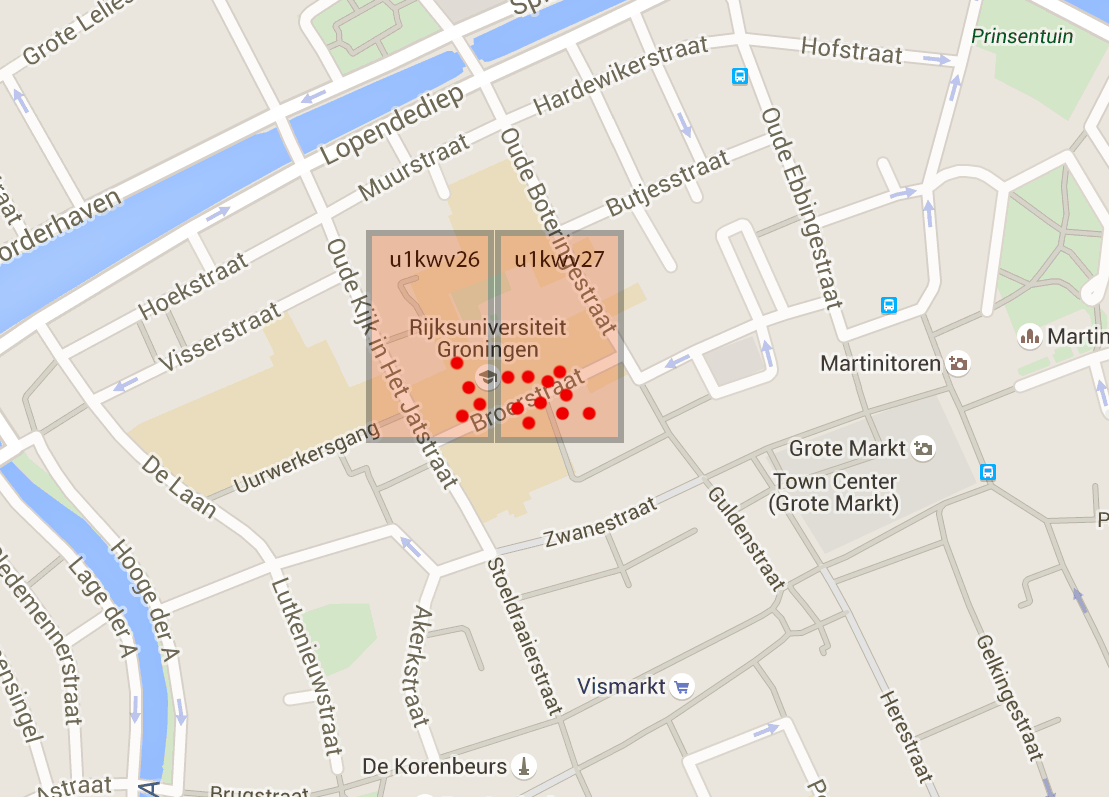
\includegraphics[width=4in]{bordercase.png} 
   \caption{Geohash border case(Red dots are tweets)}
   \label{Geohash border case}
\end{figure}

In the output from the clusterCreator.py script we be in this case two different clusters. To merge events that refer to the same event but have different geohashes (and are neighbors) we use this script to merge these cases. We do this by iterating over all clusters and calculate the neighboring geohashes. For each neigboring geohash we check if there is an cluster within the same time period. If we find a cluster with a neighboring geoHash and with the same timestamp +/- 60 minutes we calculate the word overlap because it can also be a different event that is coincidental taking place at the same time and close to current geoHash. We calculate this wordoverlap by looking at the 10 most common word in both clusters. For each word that overlaps a score of one point is awarded. If a hashtag or username overlaps two points are awarded. If a score exceeds the threshold the function returns true. The threshold is determined by experimenting with a lot of different values.\newline
We discussed the number of iterations needed because it is also possible to look at the neighbors of the neighbors but we concluded that one iteration was sufficient. The area you get when you look at the neighbors for one iterations is big enough and if you go bigger you get events that are not local.



\begin{python}
def _calculateWordOverlap(self,clusterA, clusterB):      
    wordsClusterA = self._getImportantWords(10, clusterA)
    wordsClusterB = self._getImportantWords(10, clusterB)
    result = {}
    
    #intersect the two lists and adding the scores
    for wordA, scoreA in wordsClusterA:
        for wordB, scoreB in wordsClusterB:
            if wordA == wordB:
                result[wordA] = scoreA + scoreB
                if wordA[0] == '#':
                    result[wordA] *= 2
                if wordA[0] == '@':
                    result[wordA] *= 2

    if sum(result.values()) > self.THRESHOLD:
        return True
    else:
        return False
\end{python}

The output of this script is an updated dictionary where neighboring clusters about the same event will be merged.

\paragraph{EventCandidates.py} is the wrapper class for this module. This script generates all eventCandidates using the scripts described above. This function requires two parameters. The first is the name of the text file with the unprocessed tweets. The second is the desired name of the dataset. This script saves a JSON file with all eventCandidates.

\subsection{Annotation}
We created two datasets. One for developing and one for testing. We annotated the testing dataset in the final period of our research.
The data is annotated  with an interactive tool by two judges. This tool also calculates the kappa score: was 0.79 for the development dataset and 0.8 for the test dataset. According to book IR is dat fair/good. We discarded the eventCandidates we did not agree on.

For the development dataset we annotated 1350 event candidates with these categories. In 87\% of the cases the judges agreed.

\begin{table}[h]
\caption[Confusion matrix testset annotation]{Confusion matrix development dataset annotation }
\begin{tabular}{lcccccc}
 & \multicolumn{1}{l}{\textbf{OTH}} & \multicolumn{1}{l}{\textbf{MEE}} & \multicolumn{1}{l}{\textbf{ENT}} & \multicolumn{1}{l}{\textbf{NOE}} & \multicolumn{1}{l}{\textbf{INC}} & \multicolumn{1}{l}{\textbf{SPO}} \\ \cline{2-7} 
\multicolumn{1}{l|}{\textbf{OTH}} & \multicolumn{1}{c|}{\textless1\textgreater} & \multicolumn{1}{c|}{.} & \multicolumn{1}{c|}{.} & \multicolumn{1}{c|}{2} & \multicolumn{1}{c|}{1} & \multicolumn{1}{c|}{1} \\ \cline{2-7} 
\multicolumn{1}{l|}{\textbf{MEE}} & \multicolumn{1}{c|}{21} & \multicolumn{1}{c|}{\textless207\textgreater} & \multicolumn{1}{c|}{7} & \multicolumn{1}{c|}{25} & \multicolumn{1}{c|}{.} & \multicolumn{1}{c|}{2} \\ \cline{2-7} 
\multicolumn{1}{l|}{\textbf{ENT}} & \multicolumn{1}{c|}{3} & \multicolumn{1}{c|}{.} & \multicolumn{1}{c|}{\textless20\textgreater} & \multicolumn{1}{c|}{5} & \multicolumn{1}{c|}{.} & \multicolumn{1}{c|}{.} \\ \cline{2-7} 
\multicolumn{1}{l|}{\textbf{NOE}} & \multicolumn{1}{c|}{14} & \multicolumn{1}{c|}{27} & \multicolumn{1}{c|}{18} & \multicolumn{1}{c|}{\textless619\textgreater} & \multicolumn{1}{c|}{9} & \multicolumn{1}{c|}{9} \\ \cline{2-7} 
\multicolumn{1}{l|}{\textbf{INC}} & \multicolumn{1}{c|}{1} & \multicolumn{1}{c|}{2} & \multicolumn{1}{c|}{.} & \multicolumn{1}{c|}{12} & \multicolumn{1}{c|}{\textless178\textgreater} & \multicolumn{1}{c|}{.} \\ \cline{2-7} 
\multicolumn{1}{l|}{\textbf{SPO}} & \multicolumn{1}{c|}{1} & \multicolumn{1}{c|}{.} & \multicolumn{1}{c|}{.} & \multicolumn{1}{c|}{5} & \multicolumn{1}{c|}{.} & \multicolumn{1}{c|}{\textless60\textgreater} \\ \cline{2-7} 
\end{tabular}

\end{table}

For the devset we annotated 500 event candidates with these categories. In 86\% of the cases the judges agreed.

\begin{table}[h]
\caption[Confusion matrix devset annotation]{Confusion matrix test dataset annotation }
\begin{tabular}{lcccccc}
                                  & \multicolumn{1}{l}{\textbf{OTH}}            & \multicolumn{1}{l}{\textbf{MEE}}              & \multicolumn{1}{l}{\textbf{ENT}}            & \multicolumn{1}{l}{\textbf{NOE}}              & \multicolumn{1}{l}{\textbf{INC}}             & \multicolumn{1}{l}{\textbf{SPO}}    \\ \cline{2-7} 
\multicolumn{1}{l|}{\textbf{OTH}} & \multicolumn{1}{c|}{\textless.\textgreater} & \multicolumn{1}{c|}{.}                        & \multicolumn{1}{c|}{.}                      & \multicolumn{1}{c|}{.}                        & \multicolumn{1}{c|}{1}                       & \multicolumn{1}{c|}{.}              \\ \cline{2-7} 
\multicolumn{1}{l|}{\textbf{MEE}} & \multicolumn{1}{c|}{4}                      & \multicolumn{1}{c|}{\textless110\textgreater} & \multicolumn{1}{c|}{13}                     & \multicolumn{1}{c|}{9}                        & \multicolumn{1}{c|}{.}                       & \multicolumn{1}{c|}{3}              \\ \cline{2-7} 
\multicolumn{1}{l|}{\textbf{ENT}} & \multicolumn{1}{c|}{.}                      & \multicolumn{1}{c|}{.}                        & \multicolumn{1}{c|}{\textless8\textgreater} & \multicolumn{1}{c|}{2}                        & \multicolumn{1}{c|}{.}                       & \multicolumn{1}{c|}{.}              \\ \cline{2-7} 
\multicolumn{1}{l|}{\textbf{NOE}} & \multicolumn{1}{c|}{3}                      & \multicolumn{1}{c|}{19}                       & \multicolumn{1}{c|}{4}                      & \multicolumn{1}{c|}{\textless199\textgreater} & \multicolumn{1}{c|}{4}                       & \multicolumn{1}{c|}{2}              \\ \cline{2-7} 
\multicolumn{1}{l|}{\textbf{INC}} & \multicolumn{1}{c|}{1}                      & \multicolumn{1}{c|}{.}                        & \multicolumn{1}{c|}{.}                      & \multicolumn{1}{c|}{.}                        & \multicolumn{1}{c|}{\textless78\textgreater} & \multicolumn{1}{c|}{.}              \\ \cline{2-7} 
\multicolumn{1}{l|}{\textbf{SPO}} & \multicolumn{1}{c|}{.}                      & \multicolumn{1}{c|}{1}                        & \multicolumn{1}{c|}{2}                      & \multicolumn{1}{c|}{2}                        & \multicolumn{1}{c|}{.}                       & \multicolumn{1}{c|}{\textless60\textgreater} \\ \cline{2-7} 
\end{tabular}

\end{table}




\subsection{Event detection}
For the event detection I trained two classifiers using NLTK. The first classifier trains using the words (800 most common words with stopwords removed) as features. Several values were tried but 800 resulted in the best performance. Also several types of classifiers were tried. Naive Bayes produced the best result and was also the quickest. The output of that classifier (a category) was used as a feature for the second classifier that used more features as described in the next section.
\newpage
\subsubsection{Feature selection}
The first classifier only uses the words as features. The second classifier uses the output of the first classifier as a feature. This feature is by far the most valuable for the system. In the table below the performance of the features are described. In appendix x the complete results can be found.


\begin{table}[h]
\caption[Effect of features]{Effect of features  }
\begin{tabular}{|l|l|}
\hline
                          & Accuracy \\ \hline
All features              & 0.84     \\ \hline
Category                  & 0.81     \\ \hline
Location                  & 0.51     \\ \hline
WordOverlapSimple         & 0.63     \\ \hline
WordOverlapUser           & 0.6      \\ \hline
WordOverlapUser, Category & 0.82     \\ \hline
\end{tabular}

\end{table}

\begin{description}

\item[Category]
The result of the classifier that uses the most common words as features. 

\item[Location]
The first 5 characters in the geoHash are used as a feature. It will be easier to detect events on locations were events often take place.

\item[wordOverlapSimple]
This feature is a numeric value that represents how many tweets consist of the same words. The score is calculated by counting the occurrences of each type and dividing it by the number of tweets. Hashtags get a bonus score.

\begin{python}
def _wordOverlapSimple(self, candidate):
        types = Counter()
        for tweet in candidate:
            types.update(set(tweet['tokens']))
        score = 0
        for t in types:
            if types[t] > 1:
                if t[0] == '#':
                    score += (types[t] * 2)
                else:
                    score += types[t]

        return round((score / len(candidate)) * 2) / 2
\end{python}
\newpage
\item[WordOverlapUser]
This feature calculates the overlap of types among users. The score is the highest when all users use the same words. The result is the log of the score and rounded to 0.5.

\begin{python}
def _wordOverlapUser(self, candidate):
        '''Calculate the overlap of features among users'''
        userTypes = defaultdict(list)
        types = Counter()

        for row in candidate:
            userTypes[row['user']].extend(row['tokens'])
        
        for user in userTypes:
            types.update(set(userTypes[user]))
        score = 0
        for t in types:
            if types[t] > 1: #ignore if only in one tweet
                if t[0] == '#':
                    score += (types[t] * 2)
                else:
                    score += types[t]

        if score > 1:
            s = log(float(score) * float(len(userTypes.keys()) )) 
            #return round((score * 2) / len(candidate))
            return round((s / len(candidate) )* 2 ) /2 
        else:
            return 0.0
\end{python}

\end{description}

\subsubsection{Results event detection}
The event classifier performs good. It is a few procent less then the Upper bound  of 87\%. 

\begin{table}[h]
\caption[Results using all features]{Results using all features }
\begin{tabular}{l|l|l|l|l|l|l|l|l|l|}
\cline{2-10}
                          & \multicolumn{3}{c|}{Naive Bayes}                                         & \multicolumn{3}{c|}{Maximum Entropy}                                     & \multicolumn{3}{c|}{SVM}             \\ \cline{2-10} 
                          & \multicolumn{3}{c|}{Accuracy = 84\%}                                     & \multicolumn{3}{c|}{Accuracy = 83\%}                                     & \multicolumn{3}{c|}{Accuracy = 81\%} \\ \cline{2-10} 
                          & \multicolumn{1}{c|}{P} & \multicolumn{1}{c|}{R} & \multicolumn{1}{c|}{F} & \multicolumn{1}{c|}{P} & \multicolumn{1}{c|}{R} & \multicolumn{1}{c|}{F} & P          & R          & F          \\ \hline
\multicolumn{1}{|l|}{NOE} & 0.85                   & 0.90                   & 0.88                   & 0.83                   & 0.93                   & 0.88                   & 0.85       & 0.83       & 0.84       \\ \hline
\multicolumn{1}{|l|}{SPO} & 0.77                   & 0.49                   & 0.60                   & 0.77                   & 0.49                   & 0.60                   & 0.77       & 0.49       & 0.60       \\ \hline
\multicolumn{1}{|l|}{ENT} & 0.00                   & 0.00                   & 0.00                   & 0.00                   & 0.00                   & 0.00                   & 0.00       & 0.00       & 0.00       \\ \hline
\multicolumn{1}{|l|}{MEE} & 0.76                   & 0.79                   & 0.77                   & 0.79                   & 0.74                   & 0.76                   & 0.65       & 0.81       & 0.72       \\ \hline
\multicolumn{1}{|l|}{INC} & 0.97                   & 0.97                   & 0.97                   & 0.94                   & 0.94                   & 0.94                   & 1.00       & 0.97       & 0.99       \\ \hline
\multicolumn{1}{|l|}{OTH} & 0.00                   & 0.00                   & 0.00                   & 0.00                   & 0.00                   & 0.00                   & 0.00       & 0.00       & 0.00       \\ \hline
\end{tabular}

\end{table}


The different classifiers perform almost the same. The 

\begin{table}[h]
\caption[Confusion Matrix Naive Bayes]{Confusion Matrix Naive Bayes }
\begin{tabular}{|l|c|c|c|c|c|c|}
\hline
    & \multicolumn{1}{l|}{OTH} & \multicolumn{1}{l|}{MEE} & \multicolumn{1}{l|}{ENT} & \multicolumn{1}{l|}{NOE} & \multicolumn{1}{l|}{INC} & \multicolumn{1}{l|}{SPO} \\ \hline
OTH & \textless.\textgreater   & .                        & .                        & 1.                       & .                        & .                        \\ \hline
MEE & .                        & \textless82\textgreater  & 2                        & 14                       & .                        & 12                       \\ \hline
ENT & .                        & .                        & \textless.\textgreater   & 1                        & .                        & .                        \\ \hline
NOE & .                        & 27                       & 5                        & \textless179\textgreater & 1                        & 7                        \\ \hline
INC & .                        & .                        & .                        & 2                        & \textless76\textgreater  & .                        \\ \hline
SPO & .                        & 1                        & 1                        & 2                        & 1                        & \textless16\textgreater  \\ \hline
\end{tabular}


\end{table}

\begin{table}[h]
\caption[Confusion Matrix Maximum Entropy]{Confusion Matrix Maximum Entropy }
\begin{tabular}{|l|c|c|c|c|c|c|}
\hline
    & \multicolumn{1}{l|}{OTH} & \multicolumn{1}{l|}{MEE} & \multicolumn{1}{l|}{ENT} & \multicolumn{1}{l|}{NOE} & \multicolumn{1}{l|}{INC} & \multicolumn{1}{l|}{SPO} \\ \hline
OTH & \textless.\textgreater   & 1                        & .                        & .                        & .                        & .                        \\ \hline
MEE & .                        & \textless81\textgreater  & 2                        & 7                        & 2                        & 11                       \\ \hline
ENT & .                        & .                        & \textless.\textgreater   & .                        & 1                        & .                        \\ \hline
NOE & .                        & 26                       & 5                        & \textless186\textgreater & 1                        & 7                        \\ \hline
INC & .                        & 1                        & .                        & 4                        & \textless73\textgreater  & .                        \\ \hline
SPO & .                        & 1                        & 1                        & 2                        & 1                        & \textless16\textgreater  \\ \hline
\end{tabular}

\end{table}

\begin{table}[h]
\caption[Confusion Matrix SVM classifier]{Confusion Matrix SVM classifier }
\begin{tabular}{|l|c|c|c|c|c|c|}
\hline
    & \multicolumn{1}{l|}{OTH} & \multicolumn{1}{l|}{MEE} & \multicolumn{1}{l|}{ENT} & \multicolumn{1}{l|}{NOE} & \multicolumn{1}{l|}{INC} & \multicolumn{1}{l|}{SPO} \\ \hline
OTH & \textless.\textgreater   & 1                        & .                        & .                        & .                        & .                        \\ \hline
MEE & .                        & \textless89\textgreater  & 2                        & 31                       &                          & 14                       \\ \hline
ENT & .                        & .                        & \textless.\textgreater   & .                        &                          & .                        \\ \hline
NOE & .                        & 19                       & 5                        & \textless166\textgreater & 1                        & 4                        \\ \hline
INC & .                        & .                        & .                        & .                        & \textless73\textgreater  & .                        \\ \hline
SPO & .                        & 1                        & 1                        & 2                        & 1                        & \textless17\textgreater  \\ \hline
\end{tabular}

\end{table}

\subsection{Named Entity Recognition}
The default NER tagger in NLTK is the Stanford NER classifier. This is according to many researches the best available. Unfortunately there are no classifiers trained using Dutch tweets and the performance of the available classifiers was so poor (see table x) i decided to train my own classifier. Because of limited time I decided to automatically annotate the training data creating a silver standard.

\subsubsection{Data collection}
I used the wordlists that are used in Alpino(LINK), that are four lists with dutch words categorized in (LOCATIONS, PERSONS, ORGANIZATIONS and MISC). I used those list to download tweets that at least contain one word from these lists. I then used the wordlists to annotate the tweets automatically in de the desired training data format. This resulted in a dataset of one million annotated tweets. 

\subsubsection{Training}
For training the classifier the dataset was divided in a train set and a test set. The Stanford NER tagger trained with several features, NGR


\newpage
\subsection{Results}
In this section the results of the two components, the classifier and the NER tagger are discussed.







\subsubsection{NER}
I compare my results with the standard Stanford 4 class classifier. This classifier is trained on xxx and uses the same classes as my classifier.

\begin{table}[h]
\caption[NER Classifier trained with Tweets]{NER Classifier trained with Tweets }
\begin{tabular}{|l|l|l|l|l|l|l|}
\hline
Entity       & P      & R      & F1     & TP & FP & FN   \\ \hline
LOCATION     & 0,7333 & 0,7333 & 0,7333 & 11 & 4  & 4    \\ \hline
MISC         & 0,0909 & 0,500  & 0,1538 & 1  & 10 & 1    \\ \hline
ORGANIZATION & 0,7500 & 0,8824 & 0,8108 & 15 & 5  & 2    \\ \hline
PERSON       & 0,6154 & 0,5517 & 0,5818 & 16 & 10 & 13   \\ \hline
Totals       & 0,5972 & 0,6825 & 0,6370 & 43 & 29 & 20 \\ \hline
\end{tabular}

\end{table}


\clearpage
\newpage
\section{Conclusion and discussion}
\lipsum[10]
\lipsum[10]

\newpage
\section{Appendix}

\begin{landscape}
\begin{table}[h]
\begin{tabular}{|l|l|l|l|l|l|l|l|}
\hline
                          & accuracy & geen\_event    & sport          & entertainment  & bijeenkomst    & incident       & anders         \\ \hline
                          &          & P    R    F    & P    R    F    & P    R    F    & P    R    F    & P    R    F    & P    R    F    \\ \hline
All features              & 0.84     & 0.85 0.90 0.88 & 0.77 0.49 0.60 & 0.00 0.00 0.00 & 0.76 0.79 0.77 & 0.97 0.97 0.97 & 0.00 0.00 0.00 \\ \hline
Category                  & 0.81     & 0.85 0.82 0.84 & 0.73 0.46 0.56 & 0.00 0.00 0.00 & 0.66 0.84 0.74 & 0.99 0.97 0.98 & 0.00 0.00 0.00 \\ \hline
Location                  & 0.51     & 0.49 0.94 0.65 & 0.00 0.00 0.00 & 0.00 0.00 0.00 & 0.66 0.25 0.36 & 0.50 0.06 0.11 & 0.00 0.00 0.00 \\ \hline
WordOverlapSimple         & 0.63     & 0.60 0.85 0.71 & 0.00 0.00 0.00 & 0.00 0.00 0.00 & 0.57 0.33 0.42 & 0.77 0.83 0.80 & 0.00 0.00 0.00 \\ \hline
wordOverlapUser           & 0.6      & 0.57 0.93 0.71 & 0.00 0.00 0.00 & 0.00 0.00 0.00 & 0.00 0.00 0.00 & 0.66 0.90 0.76 & 0.00 0.00 0.00 \\ \hline
wordOverlapUser, category & 0.82     & 0.86 0.83 0.85 & 0.77 0.49 0.60 & 0.00 0.00 0.00 & 0.66 0.85 0.74 & 1.00 0.97 0.99 & 0.00 0.00 0.00 \\ \hline
\end{tabular}
\end{table}
\end{landscape}


%----------------------------------------------------------------------------------------
\bibliographystyle{plain}
\bibliography{chris}
\end{document}